\section{Multicomponent heterogeneous systems}

After the study of systems where only one component was allowed we jumped to the study of multiple components having still one phase now also this last constraint has been released. Therefore, we want to understand how a general system behaves at thermodynamic equilibrium and to do that we need to start with the conditions for equilibrium itself. In fact, having now a series of possible phases and components the conditions seen in \eqref{eq:equiCond} are no longer exact, and we need to expand them as follows.
\thm{General equilibrium conditions}
{
    In a heterogeneous system with composed by $p$ phases and $c$ components we have that at equilibrium for every $\alpha$ and $\beta$ phases inside the system the following is true $\forall i \in \{0, \dots, c\}$ components
    \begin{equation}
        \label{eq:GenralEquilibriumConditions}
        T^\alpha = T^\beta, \hspace{2cm} P^\alpha = P^\beta, \hspace{2cm} \mu^\alpha_i = \mu^\beta_i. 
    \end{equation}
}
\pf{Proof}
{
    The proof is totally analogous to the one for the equilibrium conditions of the simpler case, the only difference is that now the differential of the internal energy contains more elements being
    \begin{equation}
        \dd U' = \sum_{\nu=1}^p\left( T^\nu \dd S'^\nu - P^\nu\dd V'^\nu + \sum_{i=1}^c \mu_i^\nu\dd n_i^\nu\right).
    \end{equation}
    Applying the equilibrium conditions of an isolated system that in our case are
    \begin{equation}
        \sum_\nu \dd U'^\nu = 0, \hspace{2cm} \sum_\nu \dd V'^\nu = 0, \hspace{2cm} \sum_\nu \dd n_i^\nu = 0,
    \end{equation}
    we can simply arrive to the wanted result.
}
\noindent
Basically, we need to keep in mind that more components are present and so, for two phases to be in equilibrium with each others we need that the chemical potentials of the different components are equal in both phases component by component.

The equilibrium conditions are the main general properties that are needed in order to study such systems. By keeping them in mind we can start to develop the theory of how this kind of general materials behave, understanding how the phases interacts with one another at equilibrium.

\subsection{Gibbs' phase rule}

In the construction of a phase diagram of a general system one may think that nothing is really known a priori due to the complexity of the system itself. Nevertheless, it's possible to find out some insight on at least the degrees of freedom that we have inside the diagram. In fact the equilibrium conditions gives large limitations on the possible thermodynamical variable that can change in certain regions of the phase diagram leaving us with the following result.
\thm{Gibbs' phase rule}
{
    In a system with $p$ phases and $c$ component the available degrees of freedom inside the system are given by the following relation
    \begin{equation}
        \label{eq:GibbsPhaseRule}
        f = c - P + 2.
    \end{equation}
}
\pf{Proof}
{
    We have, from \eqref{eq:GenralEquilibriumConditions}, that $T$ and $P$ must be the same for all phases, so $2$ variables are present. Then we also have the molar fractions $X_i^j$ to be possible variable having exactly $(c - 1)p$ of them, one for every component in every phase with a $-1$ due to the condition
    \begin{align}
        &\sum_i X^j_i = 1, &\forall j \in \{ 1, \dots, p \}.
    \end{align}
    Then we have the chemical potentials, which sets further restrictions to the system where we need to have all $\mu_i^1 = \dots = \mu_i^p$ for every component giving us $c(p-1)$ constrains which lead us to
    \begin{equation}
        f = 2 + (c-1)p - c(p-1) = c - p + 2,
    \end{equation}
    as expected.
}
\begin{figure}[t]
    \centering
    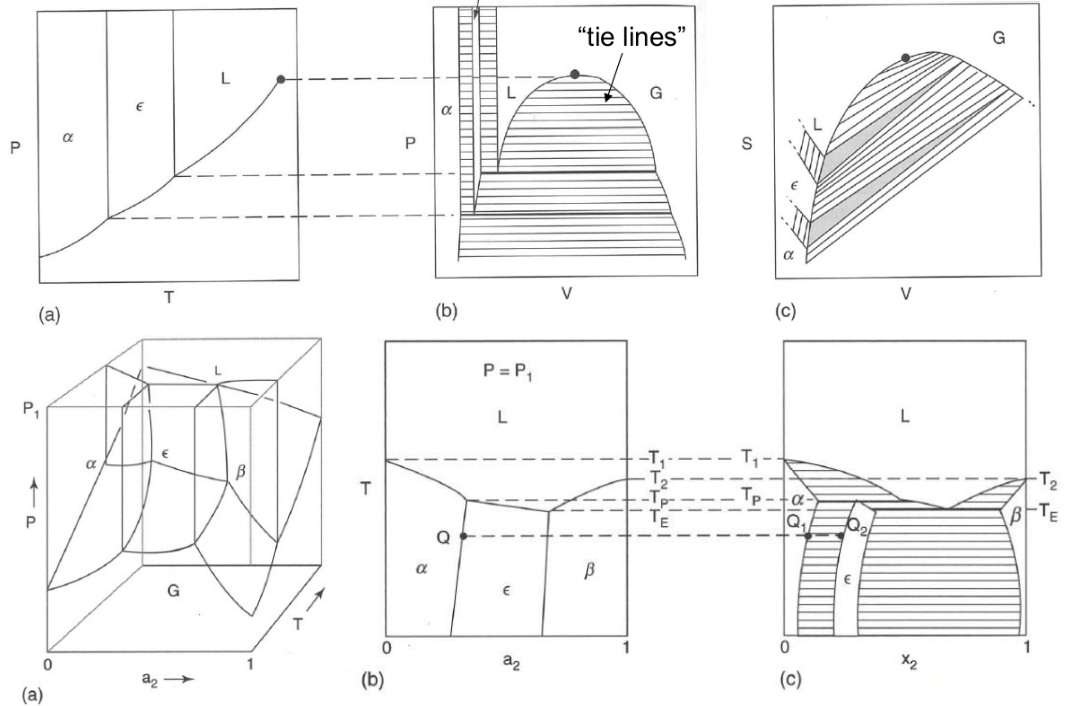
\includegraphics[width=0.8\textwidth]{Immagini/GeneralPhaseDiag.png}
    \caption
    {
        Examples of phase diagrams in different phase space for a two component, top, and a three component system, bottom. It's possible to see how the Gibbs' phase rule is respected perfectly in the $T$ vs $P$ phase space while modifications due to more freedom in the parameters are present in the others. In (b) of bottom row an isobaric section of (a) is represented.
    }
    \label{fig:GeneralPhaseDiag}
\end{figure}

\noindent
This rule is telling us a lot on the phase diagram properties in general. In fact, we can understand that in a system with two components if I want to have two phases coexist the degrees of freedom available becomes simply one, meaning that the region with two phases coexisting is a line as we know. Instead, if we want three phases zero degrees of freedom are present becoming a point, that is what we already called triple point. If we wanted to go up with the number of phases the value of $f$ will become negative, which is impossible, meaning that in a binary system only maximum three phases can coexist at once. The latter is a result that can be generalized really easily having that.
\cor{Maximum coexisting phases}
{
    In a system with $p$ phases and $c$ component the maximum number of coexisting phases are $c + 2$.
}
\noindent
Examples of this can be clearly seen inside \figref{fig:GeneralPhaseDiag} where phase diagrams of binary and ternary components are present, and we can see how in the formers the points find themselves in the connection of four phases the maximum number that can coexist.

It's also important to keep in mind that this result is valid as long as we represent the diagrams in the $(T, P)$ phase space, if we change visualization to another space the diagram will change and also the degrees of freedom can. Looking at the figure (b) in the top row of \figref{fig:GeneralPhaseDiag} we can see an example, substituting the variable $T$ with the volume $V$ makes it so that the latter can change at equilibrium since no condition on him is present inside \eqref{eq:GenralEquilibriumConditions}. Therefore, if we take a triple point and draw it on $(P,V)$ it will become a so-called \textbf{tie line} horizontal to the x-axis that allow to have the coexistence of the phases also while the volume of the system can change. That can also be seen for the $X_2$ case in the ternary component system of the bottom row where coexistent of different phases can be present at different values of molar content while in the normal representation they were points.

\subsection{Binary phase diagrams}

Let's now focus a moment on a binary heterogeneous system, a situation that we have already seen during the homogeneous study founding out that for certain interaction parameters and temperatures a miscibility gap appeared bringing the system to form two different phases. We want now to describe some features of this separation of phases using the same conceptual model used before, having that the homogeneous system separates in a phase $\alpha$ that is more rich of atoms of type $1$ and a $\beta$ rich of type $2$. Therefore, we are going to consider a system with a free energy of mixing as the one seen in \figref{fig:TwoPhase}, where it's possible to understand that the miscibility gap appear only in a certain range of temperature described by the parabola like shape found out in the phase diagram.
\begin{figure}[t]
    \centering
    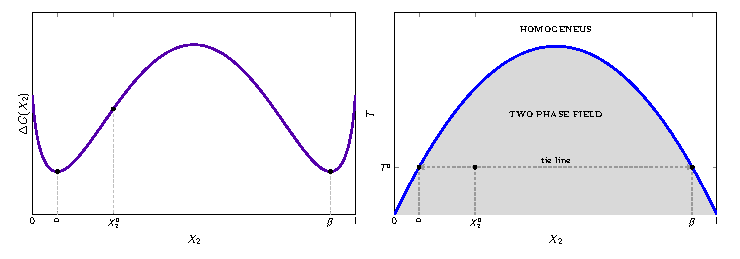
\includegraphics[width=\textwidth]{Immagini/TwoPhase.pdf}
    \caption
    {
        Illustration of a two phase system with miscibility gap, showing so a two phase field inside the phase diagram under the curve that describes the critical temperature of the system after which we have a homogeneous disordered phase. 
    }
    \label{fig:TwoPhase}
\end{figure}
The states inside that parabola forms the do called \textbf{two phase fields}, meaning that inside those states it's possible for the system to form two phases to lower the total free energy. What we want to understand now is what changes from states that are on the same tie line of the two phase field.

To answer that question we can take a system with a certain molar fraction $X_2^0$ as depicted in \figref{fig:TwoPhase} and start thinking. The system will split, since it's in the two phase field, creating zones that are in a 1-rich state $\alpha$ and others in 2-rich state $\beta$. Nevertheless, the system has in total a major number of 1 type atoms since $X_2^0$ is lower than $0.5$ meaning that it will be able to create a larger number of $\alpha$ zones. Meaning that systems on different position on the tie line will differ by the \textbf{relative extensions of the two phases}, where systems more close to $\alpha$ will have larger 1-rich zones while the other will have larger $\beta$ phases rich of 2 type atoms. It's also possible to evaluate the weights $a_\alpha$ and $a_\beta$ of the two phases inside a system by using the following relations
\begin{align}
    &a_\alpha + a_\beta = 1, &a_\alpha X_2^\alpha + a_\beta X_2^\beta = X_2^0,
\end{align}
where $X_2^i$ represent the molar fractions of the two minima. These relations form a system of equation that can be easily solved obtaining the simple solutions
\begin{align}
    \label{eq:weightPhases}
    &a_\alpha = \frac{X_2^\beta - X_2^0}{X_2^\beta - X_2^\alpha}, &a_\beta = \frac{X_2^0 - X_2^\alpha}{X_2^\beta - X_2^\alpha}
\end{align}
In this way we can understand how much total volume of the system the two phases will take for themselves. One should also notice how these results are analogous at the one found out in classical mechanics to evaluate the on the two extreme of a lever, for this reason \eqref{eq:weightPhases} are also referred to as \textbf{lever rules}.

Another important thing that we say is that by now we have always looked at the free energy of mixing, but it's also interesting to look at the normal free energy of the system depicted in \figref{fig:DoubleTang}.
\begin{figure}[t]
    \centering
    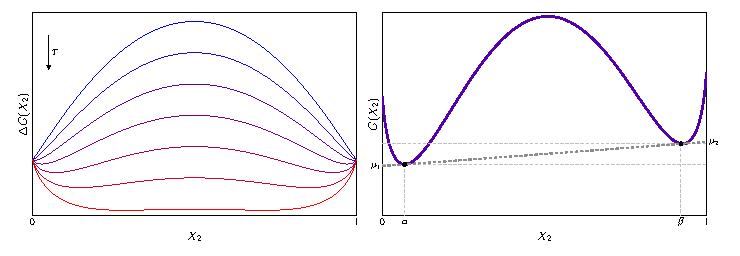
\includegraphics[width=\textwidth]{Immagini/DoubleTang.pdf}
    \caption
    {
        Representation of the mixing free energy at different temperatures on the left, and of the form of the normal free energy written as $G = \Delta G + \mu^0_2 X_2$ assuming $\mu^0_1 = 0$ on the left. It's possible to notice how the final form of $G$ is asymmetric.
    }
    \label{fig:DoubleTang}
\end{figure}
We know how the form of the free energy can be obtained from the mixing one by using the relation
\begin{equation}
    G = \Delta G + \sum_i \mu_i^0 X_i,
\end{equation}
with $\mu_i^0$ the chemical potential of the $i$-th component in its separated form. This makes so that the final form of the free energy is no more symmetric with minima that are not the same of the free energy of mixing, in fact the added terms shift the minima in others point so that they don't really represent the equilibrium phases. In fact, if we use the \textbf{tangent construction} to evaluate $\mu_i$ of the two phases, by taking the tangents in the two minima, we would have that the results, $\mu_i(X_2^\alpha)$ and $\mu_i(X_2^\beta)$, would be at different height and so the equilibrium conditions of \eqref{eq:GenralEquilibriumConditions} are not respected. Nevertheless, we can overcome this problem in a simple way by using the so-called \textbf{Double tangent construction}. 
\thm{Double tangent construction}
{
    Let $G$ be the Gibbs free energy of the system under study, to find out the minimum of $\Delta G$ we can search for two points on the curve that posses same derivative so that a tangent line connect them without crossing the graph.
}
\pf{Proof}
{
    More than a mathematical proof this is a reasoning. We know that the intercept of the tangent to a graph with the delimiting axis will give out the values of the chemical potential related to the two components inside the system. Therefore, using this construction we have found out two points that posses same intercepts, as depicted in \figref{fig:DoubleTang}, and so have the same chemical potential for the two components respectively, satisfying by construction the equilibrium conditions.
}
\noindent
Therefore, in this way the two real phases that are stable at equilibrium constituting the minima of $\Delta G$ are found graphically in a simple way analogous to the tangent construction present inside the homogeneous systems. Also, this construction works also if the system posses several Gibbs free energy of different type of phases that are contending with each other like: liquid state $G^L$, gases state $G^g$ or different types of solid phases, bcc structure, fcc and so on. All of them can be present, and you can study the ones that are in equilibrium with each other by using as the real free energy
\begin{equation}
    G(X) = \min\{ G^L(X), G^g(X), \dots \},
\end{equation}
so that the construction remains the same, only changes that more phases can be in equilibrium together.

\nt
{
    I also wanted to point out that the double tangent construction also allows to understand that the points in the middle of the two that defines the tangent constitute a miscibility gap. Having so that a two phase field is present every time the double tangent is constructed. Thus, if the point is onto the far left or the far right of the curve the system will be in a homogeneous situation since no tangent con be constructed, meaning that no other state has same chemical potential and so can be in equilibrium with it.
}


\subsection{Examples of binary phase diagrams}

At last, we can show some examples of some standard phase diagrams of binary components that may allow comprehending better the concepts shown so far while seeing how much phase diagrams can tell us on the systems we are looking at. While looking at the different examples one can also keep in mind that the most of them can be reproduced using as models for the Gibbs energy of the different phases a regular solution like
\begin{align}
    &G^L = \mu^{0,L}_1 X_1^L + \mu^{0,L}_2 X_2^L + RT(X_1^L\ln X_1^L + X_2^L\ln X_2^L) + \Omega^L X_1^LX_2^L,\\
    &G^\alpha = \mu^{0,\alpha}_1 X_1^\alpha + \mu^{0,\alpha}_2 X_2^\alpha + RT(X_1^\alpha\ln X_1^\alpha + X_2^\alpha\ln X_2^\alpha) + \Omega^\alpha X_1^\alpha X_2^\alpha.
\end{align}
Where the $\alpha$ phase usually represent a particular type of solid state. Therefore, by changing the values of $\mu_i^{0,j}$ and the interactions parameters $\Omega^j$ one should be able to obtain in good approximation all the examples we will show.

\paragraph{Isomorphous Systems.} These are systems where the Two elements are completely soluble in each other in solid and liquid states. To have two atoms be able to achieve this type of solutions they need to possess some particular characteristics called \textbf{Hume-Rothery Rules}. The latter are empirical properties that have been observed through experiments, and shows that the atoms need to have: 
\begin{align*}
    & 1)\text{ similar radii,} \hspace{4.05cm} 2)\text{ same crystal structure,}\\
    & 3)\text{ similar electronegativity,} \hspace{2cm} 4)\text{ solute should have higher valence.}
\end{align*}
The most simple example that respect those conditions is \ce{Cu-Ni} which forms a really simple system whose phase diagram is reported in \figref{fig:Cu-Ni}.
\begin{figure}[t]
    \centering
    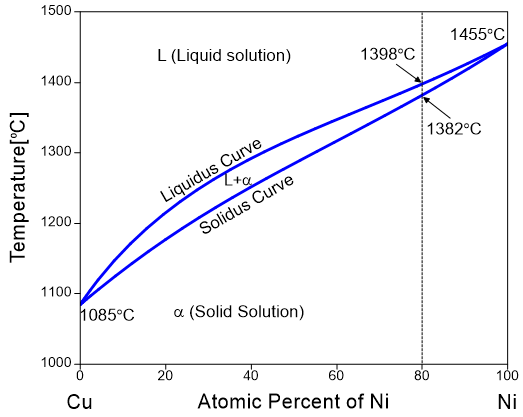
\includegraphics[width=0.6\textwidth]{Immagini/Cu-Ni.png}
    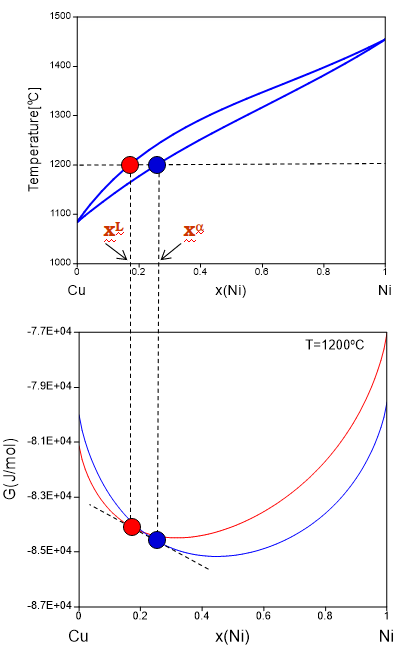
\includegraphics[width=0.3\textwidth]{Immagini/Cu-NiDoubTg.png}
    \caption
    {
        Phase diagram of \ce{Cu-Ni} system on the left, with double tangent construction of it on the right for a certain fixed temperature reported on the image. 
    }
    \label{fig:Cu-Ni}
\end{figure}
From the latter we can simply see how the system can change phase, going from an $\alpha$ solid phase to the liquid one passing through a double one where both liquid and solid exist. Nevertheless, no miscibility gap is present, meaning that there's not a portion of the phase space where the system splits in two phases that have different atomic percentage of the two components. In fact, we will give the following definition for an element to be soluble inside another.
\dfn{Solubility of an element}
{
    Inside a multicomponent system, we will tell that one element has a solubility $\gamma$ inside another element at certain temperature when, taken $X$ the molar fraction of that element in the solution, the following is true
    \begin{align}
        &X < \gamma,\text{ homogeneous}; &X > \gamma,\text{ heterogeneous}.
    \end{align}
}
\noindent
Basically, an element is soluble inside another as long as the two form a homogeneous phase mixing together, but after a certain amount a miscibility gap can be found and the system separate in two forming a heterogeneous one. That is the phenomenon from which the miscibility gap takes the name. Also, this definition shows that the system ce{Cu-Ni} is effectively miscible over all phase space.

From this type of graph we can also take other types of information, for example the marginal lines describes the behaviors of the single elements. Therefore, giving us the values of the melting points of \ce{Cu} and \ce{Ni} being at \SI{1085}{\celsius} and \SI{1455}{\celsius} respectively. Then, we can also talk about the evolution of the system as it moves inside the phase space itself, trying to understand how the system will reach equilibrium as it gets cooled or heated. Understanding this can be non-trivial, and an example of this can be seen in \figref{fig:Cu-NiEvo} where a cooling evolution is showed for a slow and quick process.
\begin{figure}[t]
    \centering
    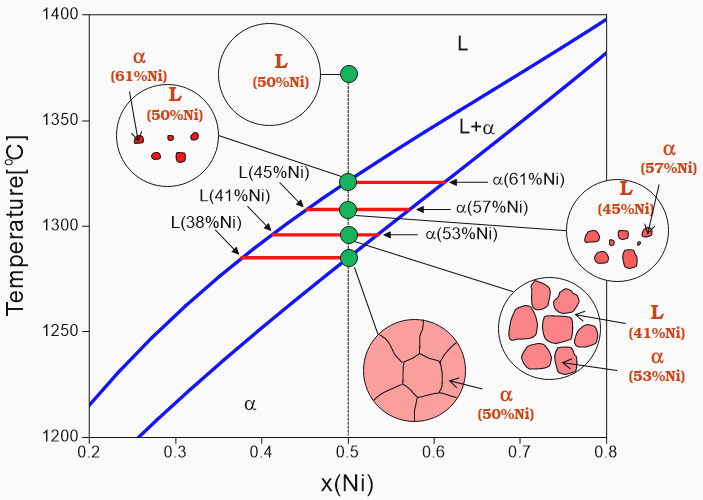
\includegraphics[width=0.47\textwidth]{Immagini/Cu-NiEvo.png}
    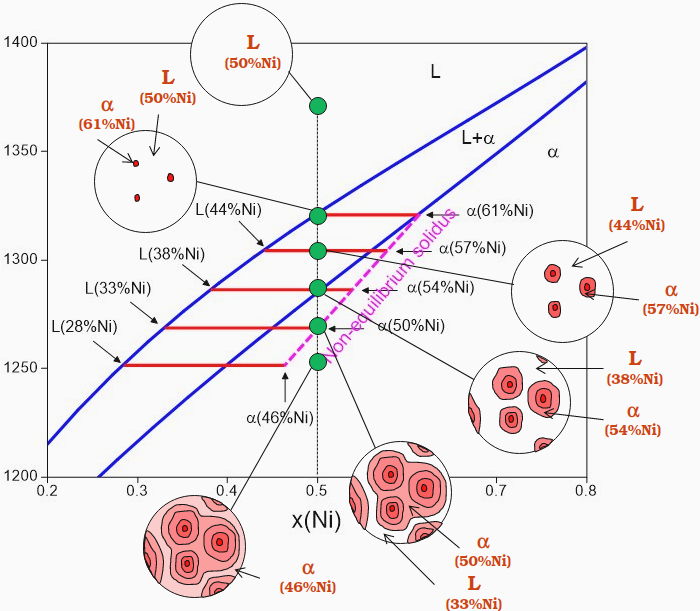
\includegraphics[width=0.39\textwidth]{Immagini/Cu-NiEvoQuick.png}
    \caption
    {
        Illustration of the cooling of the system from the liquid phase to the solid one using a slow process, on the left, and a quick one where system as no time to reach equilibrium at every step, on the right.
    }
    \label{fig:Cu-NiEvo}
\end{figure}
In the slow case the system has time to reach equilibrium at every step, entering the most favorable phase for that position in the phase space. Meaning that, from a starting liquid solution grains of solid phase with varying dimensions will start to form, and as we go down the weight $a_\alpha$ of the solid phase will start to increase following the \textbf{lever rule} having at the end only solid phases. One can also notice, from the labels in \figref{fig:Cu-NiEvo}, that the percentage of \ce{Ni} in the grains changes, that is due to the fact that as we go down in temperature also the position of the phase $\alpha$ changes moving from a higher molar fraction of Nickel to a lower one that becomes equal to the one present in the total system. Instead, in the case where the evolution goes fast the system has no time to reach equilibrium at every point, leading to the system \textbf{not completely following the phase diagram}, since it being a result of equilibrium thermodynamic can be incorrect when the processes are irreversible. In fact, in this situation as we cool down the system grains starts to form, but they are not able to form fast enough so that some liquid can remain confined inside a grain itself having so a mixture of liquid and solid also at lower temperatures respect to the expected one. This interesting phenomenon is also called \textbf{over-cooling}, and we will understand it better further in the course when we will talk about irreversible thermodynamic.

\paragraph{Eutectic Systems.} This type of system are characterized by the presence of a particular triple point inside the phase diagram called \textbf{Eutectic point} connecting a liquid phase to a mixture of two solid phases. We have seen two example of compounds with such phase diagrams \ce{Cu-Ag} and \ce{Pb-Sn}, still we are going to focus on the latter and look at the evolution of the system during cooling as we have done for the isomorphous systems. In particular, the phase diagram we are interested in is shown in \figref{fig:Pb-SnEvo} where also various type of systems evolution were shown. The most interesting is the one where the cooling pass through the eutectic point, top left figure, there the system goes from liquid to two solid phases in one go. Also, this process happens in a specific way, generating the two phases one next to each others in a stripe form, as depicted in figure, that is typical of the eutectic systems. We can also see how the evolution of the system away from the point is totally analogous to the one described previously by the isomorphous case only that another phase appears inside the solid one once it's formed. At last, it's possible to see how near the eutectic point the system undergoes a cooling that brings to results similar to the one of the first case, but since it first needs to create a solution with both liquid and solid grains of only one type of phase the final striped form will start to generate around the grains. Meaning that the final form will be composed by grains with both phases in it surrounded by the stripe compound typical of eutectic points.

\begin{figure}[t]
    \centering
    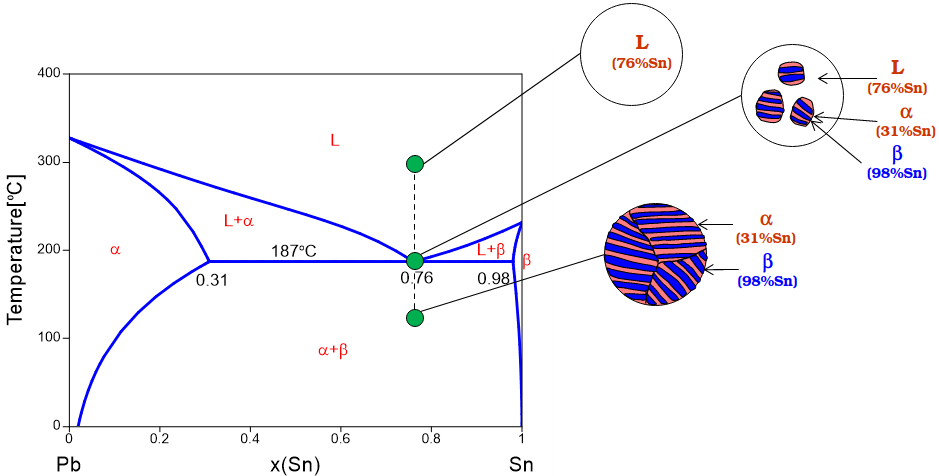
\includegraphics[width=0.45\textwidth]{Immagini/Pb-SnEvo1.png}
    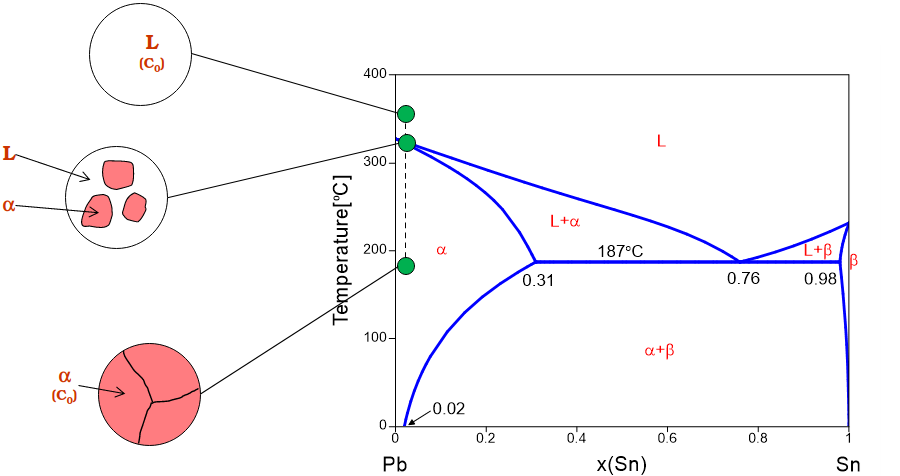
\includegraphics[width=0.45\textwidth]{Immagini/Pb-SnEvo2.png}
    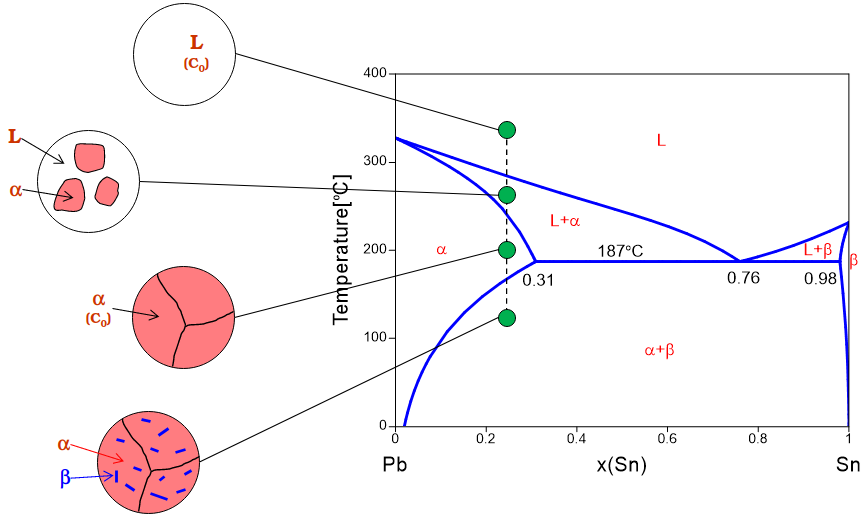
\includegraphics[width=0.45\textwidth]{Immagini/Pb-SnEvo3.png}
    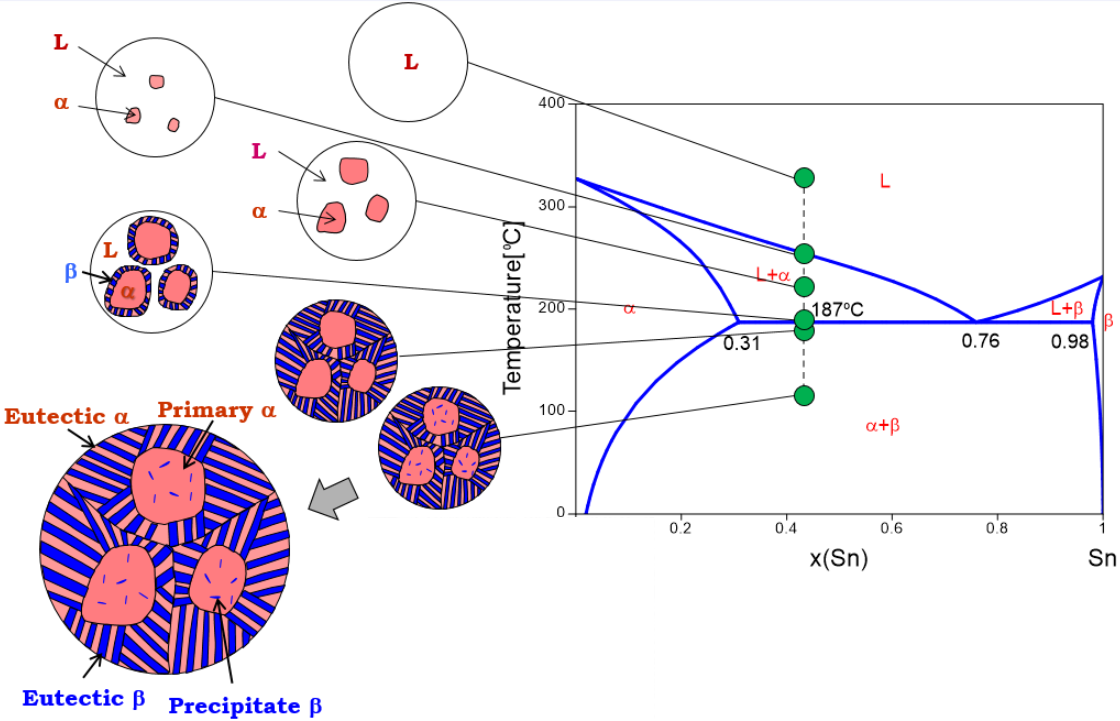
\includegraphics[width=0.45\textwidth]{Immagini/Pb-SnEvo4.png}
    \caption
    {
        Illustration of the cooling of a Eutectic system in different points of the phase diagram, looking at positions near the eutectic point and away from it.
    }
    \label{fig:Pb-SnEvo}
\end{figure}

\paragraph{Eutectoid Systems.} This type of systems are characterized by the presence of a triple point similar to the one of the eutectic systems, but it collects now a homogeneous solid phase to a heterogeneous one. 
\begin{figure}[b]
    \centering
    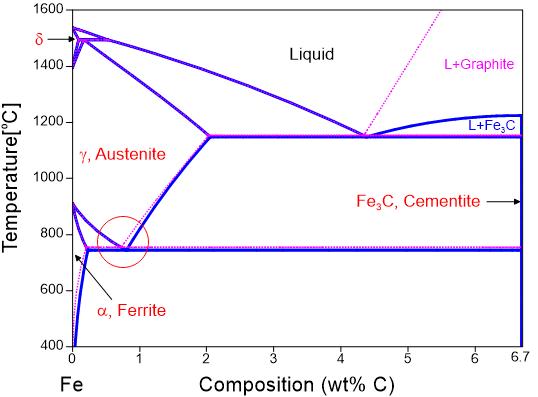
\includegraphics[width=0.35\textwidth]{Immagini/Fe-C.png}
    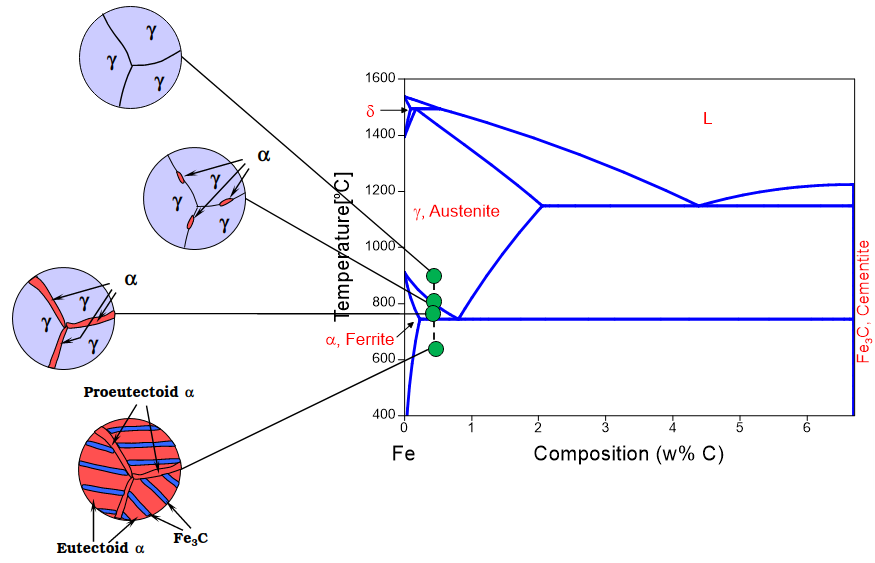
\includegraphics[width=0.4\textwidth]{Immagini/Fe-CEvo.png}
    \caption
    {
        Phase diagram of Iron-Carbon system expressed in weight percentage of Carbon. On the left the phase diagram is shown along with the real equilibrium theoretical one in pink, the difference from equilibrium are present since the mixture is in reality a metastable state that take a long time to go into real equilibrium. On the right the cooling evolution near the eutectoid point is shown. 
    }
    \label{fig:Fe-C}
\end{figure}
This system is particular to begin with, from \figref{fig:Fe-C} we can see that it possess a phase called Cementite that exist only for a really narrow part of phase space. This type of phases are known in physics as \textbf{line phases} since in the phase diagrams are basically lines meaning that they can exist only at really specific composition of the systems. Basically if we see Cementite in our system we perfectly know the Carbon weight percentage in it, which can be an interesting thing to know.

Instead, if we talk about the evolution of the system on cooling not so much changes respect to the eurectic systems. In fact, as the system pass through the eutectoid point the evolution bring to the formation of stripes as in previous case, but now they have different sizes for \ce{Fe} and \ce{C} due to the different percentage of the element in the overall material. The only real interesting thing that we can see here is when the system passes near the critical point and the intermediate solid phase, in this case $\gamma + \alpha$, needs to form in the system. That is interesting because we can see how the \textbf{new solid phase tend to form between the grain boundaries} of the $\gamma$ phase, a behavior that is common for nucleation as we will see while studying kinetics.

\nt
{
    Another series of types of binary systems is present in nature, but they all differ mainly from the type of phases that the triple point inside the phase diagram connects and on the direction of the ramifications from the point. Therefore, very little changes respect to what was sad in the previous three cases. Still, I will report on \tabref{tab:TabSys} the various possible type of systems with the different peculiar points on the phase diagrams for the ones that are more interested.
}

\begin{table}
    \centering
    \caption
    {
        Tables with all the possible type of binary systems known along with the peculiar points that characterize them inside the phase space. Also, a series of examples are reported in order to allow the reader to search for the respective phase diagram online. Notice how the ones that ends in "tectic" has liquid phase involved, while the ones in "tectoid" only posses solid phases in the equations.
    }
    \label{tab:TabSys}
    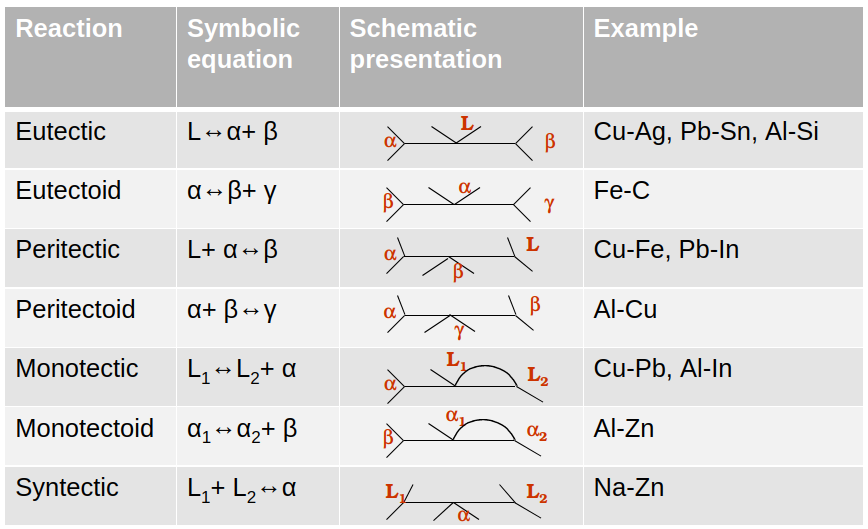
\includegraphics[width=0.6\textwidth]{Immagini/TabSyst.png}
\end{table}

\ex{Growth of nanowire}
{
    An interesting example of useful phase diagrams can be in the understanding of reality we can have a look at a really important application in the field of nanoscience, the growth of nanowire. Basically, from the phase diagram of \ce{Ge-Au}, shown in \figref{fig:Ge-Au}, one can see how the two elements are highly immiscible at normal temperature, so that really the solubility of the two is basically zero. Nevertheless, at higher temperature the liquid phase is perfectly homogeneous, so that by heating up the mixture we can create a solution where the two elements are coexisting homogeneously. Still, when the liquid mixture is obtained we can increase the percentage of Germanium inside it bring the system inside the two phase field on the left, starting the nucleation of Germanium inside the mixture. Knowing this we can simply take a substrate of \ce{Si} and place liquid \ce{Ge-Au} in small droplet on it as Germanium is inserted inside the chamber. In this way the \ce{Ge} concentration will increase inside the droplet and Germanium start to nucleate inside it depositing onto the substrate under the droplet growing and forming the nanowire overtime.
}

\begin{figure}[t]
    \centering
    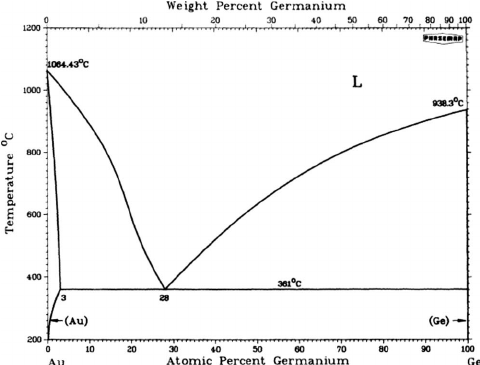
\includegraphics[width=0.35\textwidth]{Immagini/Ge-Au.png}
    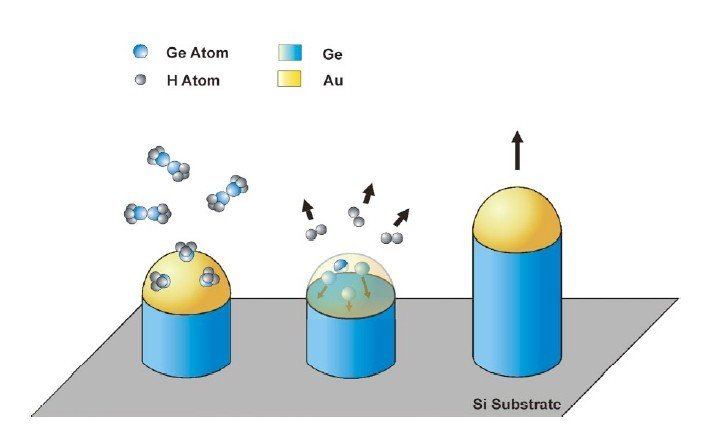
\includegraphics[width=0.45\textwidth]{Immagini/NanoGrowth.png}
    \caption
    {
        Phase diagram of \ce{Ge-Au} mixture showing how the two elements are immiscible at normal temperature with a eutectic point at $28\%$ of Germanium, on the left. Visualization of the Ge nanowire growth, on the right.
    }
    \label{fig:Ge-Au}
\end{figure}

\subsection{Quick introduction to ternary phase diagrams}

Inserting another component inside the system highly complicates the visualization of the phase diagram since a two-dimensional visualization is needed, but the presence of two independent, $X_2$ and $X_3$,  molar fractions makes a three-dimensional one more suited. The main way in which this can be overcome is usually by writing down the diagram at constant pressure and temperature so that the independent variables are only $X_2$, $X_3$, something not different from the constant pressure representation that was used in every binary phase diagram seen so far. Nevertheless, even fixed a point on $(T,P)$ phase space the visualization is complicated since the values of $X_2$ and $X_3$ are not completely uncorrelated since if $X_2 = 0.2$ the other independent variable is confined to $X_3 \in [0, 0.8]$, so can't have all possible values.
\begin{figure}[b]
    \centering
    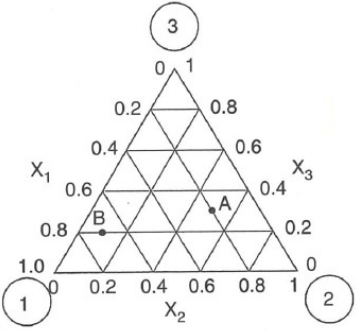
\includegraphics[width=0.3\textwidth]{Immagini/GibbsTriangle.png}
    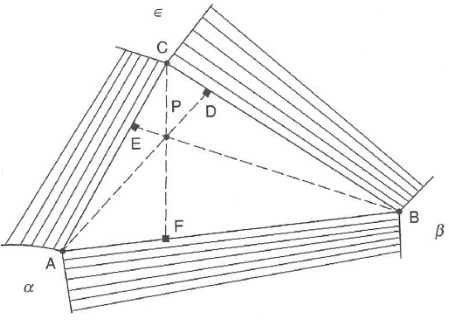
\includegraphics[width=0.35\textwidth]{Immagini/LeverRule.png}
    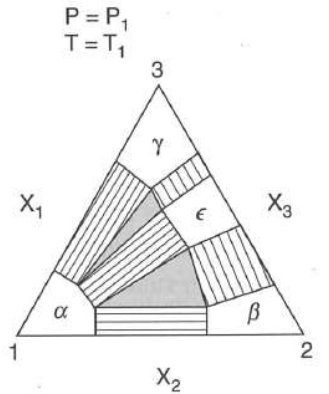
\includegraphics[width=0.24\textwidth]{Immagini/TernPD.png}
    \caption
    {
        From the left: Gibbs triangle representation of the ternary systems' phase space, example of the lever rule in a three phase field portion of the phase space, and example of a ternary phase diagram.
    }
    \label{fig:TernaryPD}
\end{figure}
To overcome this problem a cleaver graphical representation of the phase diagram is used called \textbf{Gibbs triangle}, showed in \figref{fig:TernaryPD}, where the phase space is seen as an equilateral triangle. Inside this representation to find out the molar fraction $X_i$ of a component of a point in phase space the following procedure need to be used:
\begin{enumerate}
    \item[1)] On the point, draw the line perpendicular to the median that begin from the vertex that correspond to the $i$-th component you are interested in;
    \item[2)] See where it intersects the side of the triangle corresponding to $X_i$, the point found is its value.
\end{enumerate}
In this way we are able to define the molar fraction of every point inside the system so that the sum of all $X_i$ gives out $1$.

Using Gibbs triangle we are, therefore, able to visualize in a simple two-dimensional way the phase diagrams of all ternary systems at constant $T$ and $P$, where an example is given inside \figref{fig:TernaryPD}. In the latter we can also see how, due to the present of three component, ternary phase fields now appears along the binary phase ones, forming triangular shapes inside the phase diagram. We have already seen how to treat the binary phase field, in particular the weight of the two components inside the heterogeneous phase using the \textbf{lever rule}. It's possible to see how a form of the lever rule can be found also inside this more complex situation, where the weights of the three possible phases can be evaluated using the lengths of the lines that connects the points to the vertices corresponding to a determinate phase. In particular, using as reference \figref{fig:TernaryPD}, the following relations can be obtained
\begin{equation}
    a_\alpha = PD/AD, \hspace{2cm} a_\beta = PE/BE, \hspace{2cm} a_\epsilon = PF/CF,
\end{equation}
giving the relative extensions of the three phases inside the system we are studying. Obviously, this is only the tip of the iceberg since the complexity of the ternary phase diagrams goes far beyond this and a lot of other aspects could be described. Nevertheless, this is not a course purely on phase diagram study, and so the full description of ternary, along with quaternary and so on, case goes beyond its scope. For this reason we will stop to this simple description on the Gibbs' representation and the lever rule.